\section{Results}
In this short section we will revisit the model of \cite{huberman_evolutionary_1993} mentioned in the introduction and present results simulating it with our four update-strategies. 

\begin{figure*}
        \centering
        \begin{subfigure}[b]{0.475\textwidth}
            \centering
            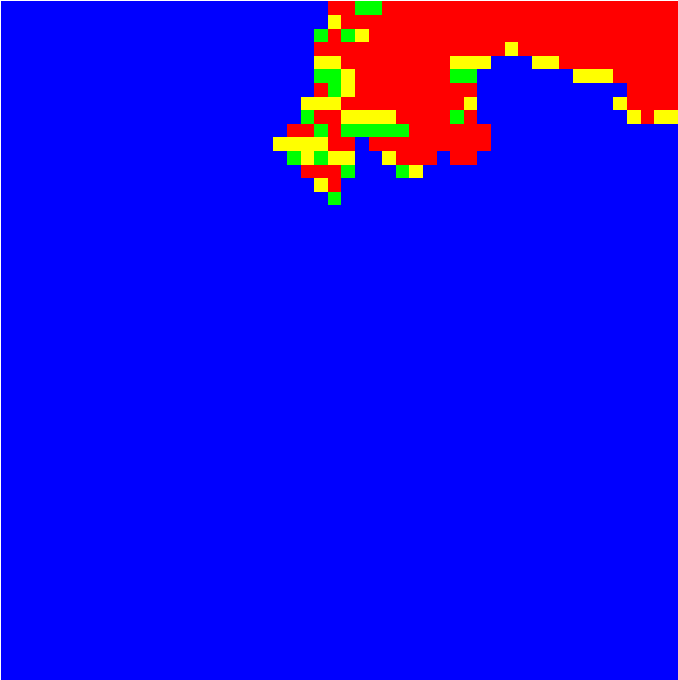
\includegraphics[width=.4\textwidth, angle=0]{./fig/seq_50x50_45steps_MSG_haskell.png}
            \caption[]%
            {{\small Sequential Strategy}}    
            \label{fig:seq_strat}
        \end{subfigure}
        \hfill
        \begin{subfigure}[b]{0.475\textwidth}  
            \centering 
            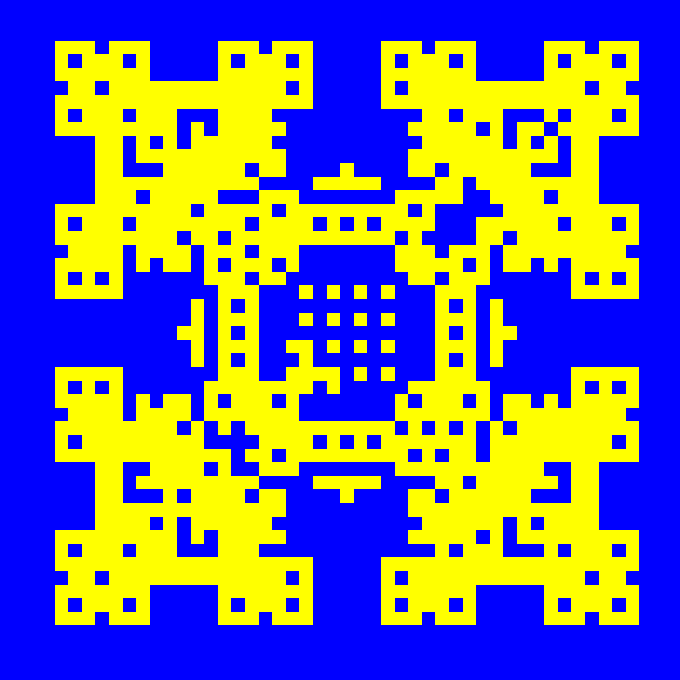
\includegraphics[width=.4\textwidth, angle=0]{./fig/par_50x50_45steps_MSG_haskell.png}
            \caption[]%
            {{\small Parallel Strategy}}    
            \label{fig:par_strat}
        \end{subfigure}
        \vskip\baselineskip
        \begin{subfigure}[b]{0.475\textwidth}   
            \centering 
            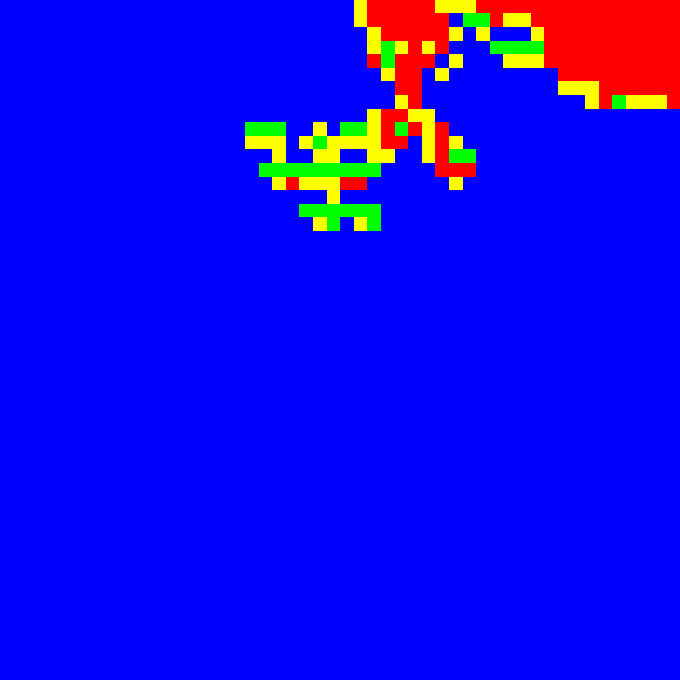
\includegraphics[width=.4\textwidth, angle=0]{./fig/con_50x50_45steps_MSG_haskell.png}
            \caption[]%
            {{\small Concurrent Strategy}}    
            \label{fig:con_strat}
        \end{subfigure}
        \quad
        \begin{subfigure}[b]{0.475\textwidth}   
            \centering 
            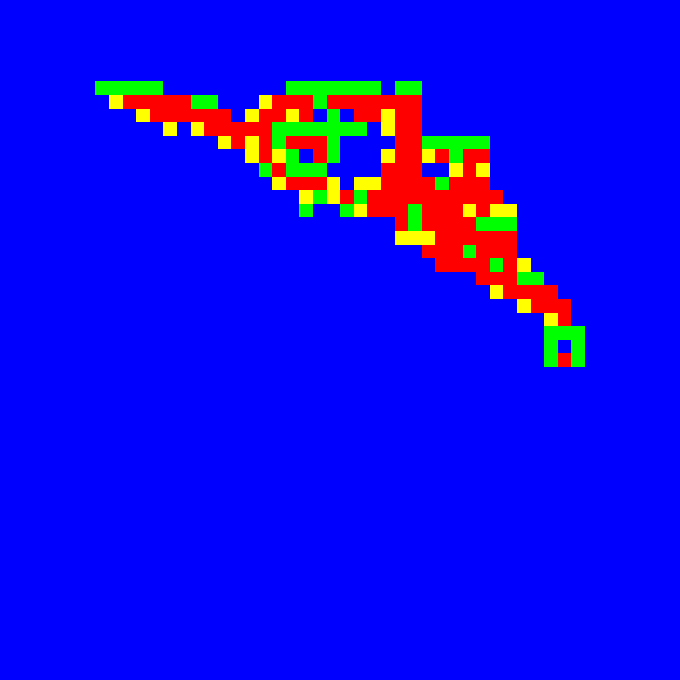
\includegraphics[width=.4\textwidth, angle=0]{./fig/act_50x50_45steps_MSG_haskell.png}
            \caption[]%
            {{\small Actor Strategy}}    
            \label{fig:act_strat}
        \end{subfigure}
        \caption[]
        {\small Haskell implementation of Prisoner-Dilemma game as in \cite{huberman_evolutionary_1993} on a 50x50 grid after 45 steps.} 
        \label{fig:prisoner_strategies}
    \end{figure*}
    
It is immediate clear that, when looking at figure \ref{fig:prisoner_strategies} the update-strategy which reflects the semantics of the model is the Parallel Strategy as all others clearly fail to reproduce the pattern as predicted by the model. Thus we can say only the Parallel Strategy is suitable to simulate this model and that only this Strategy is the correct one. \\
The reason why the others fail to reproduce the pattern is due to the non-parallel and unsynchronized way that information spreads through the grid: in the Sequential Strategy the Agents further ahead in the queue play the game earlier and influence the neighbourhood thus Agents in the neighbourhood which play the game later find an already changed environment/messages and act thus based upon these informations. This is not the case in the Parallel version: all Agents play the game on the frozen state of the previous step and the outcome of each Agents game will only be visible in the next step. In the Concurrent and Actor Strategy the Agents run in parallel but changes are visible immediately and concurrently, thus leading to the same non-structural patterns as in the Sequential Strategy. \\
Note that the Concurrent and Actor Strategy produce different results on every run due to the inherent non-deterministic event-ordering introduce by concurrency. Also note that it is not possible to calculate 45 steps for the Actor Strategy as it lacks the Global Synchronization property. To arrive at a relative comparative result we just waited until the first Agent arrives at a local time of 45 and then rendered the result. 